% !TEX program = XeLaTeX
% Standalone version of the top-tier system spine from poster.tex.
% Output: figures/pico_spine.pdf  — for the PICO pitch title slide.
\documentclass[border=10pt]{standalone}
\usepackage{fontspec}
\usepackage{xcolor}
\usepackage{tikz}
\usetikzlibrary{arrows.meta, positioning, shapes.geometric}

\setmainfont[
  Path=resources/fonts/,
  Extension=.ttf,
  BoldFont=*bd,
  ItalicFont=*i,
  BoldItalicFont=*bi
]{arial}

\definecolor{darkgray}{HTML}{232834}

\begin{document}
\begin{tikzpicture}[
    font=\fontsize{40}{48}\selectfont,
    box/.style={rectangle, rounded corners=6pt, draw=darkgray, line width=1.4pt,
                fill=white, align=center, minimum width=12cm, minimum height=5.5cm},
    arrow/.style={-{Latex[length=4.5mm, width=3.2mm]}, line width=1.5pt, draw=darkgray},
    flowlabel/.style={font=\fontsize{28}{34}\selectfont, align=center, fill=white,
                      inner xsep=3pt, inner ysep=2pt}
  ]
    \node[box] (rocket) at (7,0)    {Rocket};
    \node[box] (ipp)    at (36.5,0) {Impact Point\\Prediction System};
    \node[box] (asv)    at (66,0)   {ASV};

    \draw[arrow] (rocket.east) -- (ipp.west)
      node[midway, above=8pt, flowlabel] {sensor data};
    \draw[arrow] (ipp.east) -- (asv.west)
      node[midway, above=8pt, flowlabel] {predicted impact point\\and covariance};
\end{tikzpicture}
\end{document}
